%%%%%%%%%%%%%%%%%%%%%%%%%%%%%%%%%%%%%%%%%
% Short Sectioned Assignment
% LaTeX Template
% Version 1.0 (5/5/12)
%
% This template has been downloaded from:
% http://www.LaTeXTemplates.com
%
% Original author:
% Frits Wenneker (http://www.howtotex.com)
%
% License:
% CC BY-NC-SA 3.0 (http://creativecommons.org/licenses/by-nc-sa/3.0/)
%
%%%%%%%%%%%%%%%%%%%%%%%%%%%%%%%%%%%%%%%%%

%----------------------------------------------------------------------------------------
%   PACKAGES AND OTHER DOCUMENT CONFIGURATIONS
%----------------------------------------------------------------------------------------

\documentclass[paper=a4, fontsize=11pt]{scrartcl} % A4 paper and 11pt font size

\usepackage[T1]{fontenc} % Use 8-bit encoding that has 256 glyphs
\usepackage{fourier} % Use the Adobe Utopia font for the document - comment this line to return to the LaTeX default
\usepackage[english]{babel} % English language/hyphenation
\usepackage{amsmath,amsfonts,amsthm} % Math packages

\usepackage{lipsum} % Used for inserting dummy 'Lorem ipsum' text into the template

\usepackage{graphicx} % Required for including pictures
\usepackage{wrapfig}
\usepackage{float}

\usepackage[top=.9in, bottom=.9in, left=1in, right=1in]{geometry}
\usepackage{hyperref}

\usepackage{sectsty} % Allows customizing section commands
\allsectionsfont{\normalfont\scshape} % Make all sections centered, the default font and small caps

\usepackage{fancyhdr} % Custom headers and footers
\pagestyle{fancyplain} % Makes all pages in the document conform to the custom headers and footers
\fancyhead{} % No page header - if you want one, create it in the same way as the footers below
\fancyfoot[L]{} % Empty left footer
\fancyfoot[C]{} % Empty center footer
\fancyfoot[R]{\thepage} % Page numbering for right footer
\renewcommand{\headrulewidth}{0pt} % Remove header underlines
\renewcommand{\footrulewidth}{0pt} % Remove footer underlines
\setlength{\headheight}{0pt} % Customize the height of the header

\numberwithin{equation}{section} % Number equations within sections (i.e. 1.1, 1.2, 2.1, 2.2 instead of 1, 2, 3, 4)
\numberwithin{figure}{section} % Number figures within sections (i.e. 1.1, 1.2, 2.1, 2.2 instead of 1, 2, 3, 4)
\numberwithin{table}{section} % Number tables within sections (i.e. 1.1, 1.2, 2.1, 2.2 instead of 1, 2, 3, 4)

\setlength\parindent{0pt} % Removes all indentation from paragraphs - comment this line for an assignment with lots of text

\graphicspath{{./graphics/}} % Specifies the directory where pictures are stored

%----------------------------------------------------------------------------------------
%   TITLE SECTION
%----------------------------------------------------------------------------------------

\newcommand{\horrule}[1]{\rule{\linewidth}{#1}} % Create horizontal rule command with 1 argument of height

\title{ 
\normalfont \normalsize 
\textsc{6.885 From ASCII to Answers} % Your university, school and/or department name(s)
\horrule{0.5pt} % Thin top horizontal rule
\large The Librarian: Entity Identification Across Media Types % The assignment title
\horrule{1pt} % Thick bottom horizontal rule
}

\author{Joshua Blum, Nolan Eastin \\ \{joshblum, neastin\}@mit.edu}

\date{\normalsize\today} % Today's date or a custom date
\begin{document}

\maketitle % Print the title

\section{Motivation}
%------------------------------------------------
Entity identification is nontrivial and especially difficult when dealing with large entities. The Librarian aims to perform automated entity identification across various media types. Given sets of text, audio, image, and video files, The Librarian can merge the sets of entities by identifying files, gathering metadata from trusted sources, (i.e. IMDB, Rotten Tomato, and Spotify APIs), and categorizing the media based on the metadata that is found. \\

The motivation behind the system is to handle large dumps of data as well as incremental updates over a large corpus of files with many contributers. The Librarian serves as a background system upon which clients can be built which handle user interaction to add and modify data within the system. An example is having a client that accepts torrent files which are then given to The Librarian for ingestion or a client that offers crowd sourced resolution based on the automated identification results.\\

The initial system has been tested with approximately 2 TB of seed data that has been collected from several sources. This data was used as training data for testing and developing our identification algorithms. Only movie entities were categorized from this corpus, although the matching algorithms can be extended to work with other media entity types. The design discusses these possible extensions, although the actual implementation of these handlers will be part of future work.\\

In addition to trying to resolve two entities algorithmically, crowd sourcing can be used to establish ground truth where necessary. If there are multiple matches for a single entity, a user can select the correct metadata for the entity or input their own. The Librarian offers a network interface for modifications to the metadata which a crowd sourcing client could be built on.\\

We begin by discussing related work (\ref{sec:related-work}), providing a system design overview (\ref{sec:system-overview}), showing an analysis of the system's performance (\ref{sec:evaluation}), list goals for future work (\ref{sec:future-work}), and discuss the conclusions of the project (\ref{sec:conclusion}).

\section{Related Work}
\label{sec:related-work}
%------------------------------------------------

\subsection{Shazam}
\label{sec:shazam}

Shazam is a widely known service that specializes in identifying songs by creating audio fingerprints from (noisy) audio samples. By using a large seed database of fingerprints, Shazam is able to establish ground truth for their matching. \\

Users provide a ten second audio sample to be fingerprinted and matched against their data set. An important part of their service is that they have the ability to use the service even with background noise. Shazam uses different filtering algorithms to reduce background noise and get better samples. Shazam also optimizes storage costs by fingerprinting audio samples based on tone intensity, which allows them to get more representative fingerprints. \\

\subsection{Audible Magic}
\label{sec:audible-magic}

Similar to Shazam, Audible Magic has a large collection of data that allows users to query audio from video files such as TV shows and movies and provide pay per use SDKs. Most of their utility comes from having a large collection of data and having large amount of fingerprints that they leverage as a service. Although open source databases containing audio fingerprints are readily available online, video fingerprinting does not have the same amount of open data. \\

\section{System Overview}
\label{sec:system-overview}

The Librarian is architected to accept jobs over a local HTTP Python Flask server and ingest them into the system. A job, which consists of a single entity to be identified, is passed through the data pipeline outlined in Figure \ref{fig:system-overview}. First, the job is queued and then consumed by a worker process. Worker processes then determine the entity type and apply a handler for this type. The system currently only accepts movie entities; however, this can extended to allow multiple handlers by using file extensions to differentiate entity types. A handler type then performs two steps to ingest the entity: first a deduplication step, and then, if the entity is not a duplicate, an identification step. Deduplication looks at the internal metadata store of The Librarian whereas identification looks at outside sources to establish ground truth. \\


\begin{figure}[H]
\center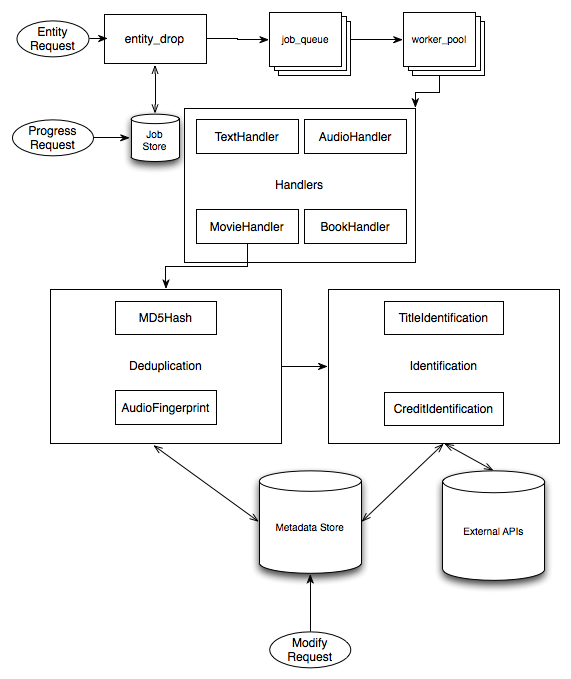
\includegraphics[scale=0.75]{system-overview.png}
\caption{The Librarian System Pipeline Overview. An entity request starts the flow through the system by 1. Creating a job for the entity. 2. Applying a handler for the entity. 3. Trying to identify the entity by deduplication or entity specific identifier method. 4. Adding the metadata found to the metadata store.}
\label{fig:system-overview}
\end{figure}


After deduplication or identification, the job is linked to an object in the metadata store. The metadata store and job store are backed by a MongoDB database. This was chosen to allow flexible schemas during development and direct storage of JSON objects obtained by external APIs. The job store can be queried with a job identification number for updates on the progress in the system or to place a modification request to manually update the metadata associated with an entity. \\

%------------------------------------------------

\subsection{Deduplication}
\label{sec:deduplication}
Deduplication is the first step in the ingestion process where the system looks for a match internally. Based on the entity type, a variety of deduplication methods can be applied. Currently hashing and audio fingerprinting are used to resolve movie entities. These methods were picked for their computational efficiency and ability to identify duplicates without requiring exact matching. \\

\subsubsection{Movie Entities}
\label{sec:dedup-movie-entities}
The deduplication process for movie entities consists of two steps. First, an md5 hash is computed across the contents of the file and the metadata store is checked for any matches. This approach is inflexible since duplicate entities can still appear. For example, if two instances of the same film are added with different video resolutions, a simple hash will produce a false negative. A more flexible but computationally expensive approach is to use audio fingerprinting. We compute a fingerprint across a subsection of the file (the first ten minutes). Only a subsection is needed since with a short duration a match can be made. Additionally, this optimization is necessary since the running time for computing a fingerprint across the entire file increases nonlinearly with file size. \\

Audio fingerprinting also has a large potential for identifying files, but requires extensive ground truth data. Shazam and Audible Magic are good examples of such services, however, their services are closed or pay per use. During the design stage we looked into fingerprinting movie trailers and checking increments of the films against these fingerprints. Yet, after some research, this method did not seem either computationally efficient nor feasible since the fingerprint requires a minimum duration of approximately ten seconds to effectively match an entity. \\

Although we were not able to use audio fingerprinting for identifying new files because we lacked ground truth data, fingerprinting proved quite effective for deduplication. We used the open source audio fingerprinting system Echoprint together with ffmpeg to extract the audio from video files and generate fingerprints. This method is very robust for deduplication since the fingerprinting algorithms allow noisy matching, making this method much more flexible than simple content hashing. \\


%------------------------------------------------

\subsection{Identification}
\label{sec:identification}
Unlike deduplication, identification is used to establish the identity of a file by looking at outside sources. These sources are assumed to have valid ground truth data which can be queried based on certain features of the file. For movie entities, the identification methods return a set of possible titles to query outside sources for metadata. For analysis purposes, all identification methods were used when matching an entity. In future iterations, once identity is established, the handler can return after a single positive identification. This design allows the author of a handler to prioritize how different identification methods are run to optimize for performance. To establish the identity of movies two identifiers were used, title identifiers and credit identifiers. \\

\subsubsection{Title Identifiers}
\label{sec:title-identifier}

The flow if the title identification algorithm is shown in Figure \ref{fig:title-identifier}. First, the title is tokenized by splitting the string on alphanumerics and we attempt to extract year information, if present. After removing any stop words, the cleaned title is checked against an internal database of known movie titles. Exact and a fuzzy matches are performed with the cleaned title. Possible matches are then queried against online sources, such as IMDB, to acquire identity metadata. \\


\begin{figure}[H]
\center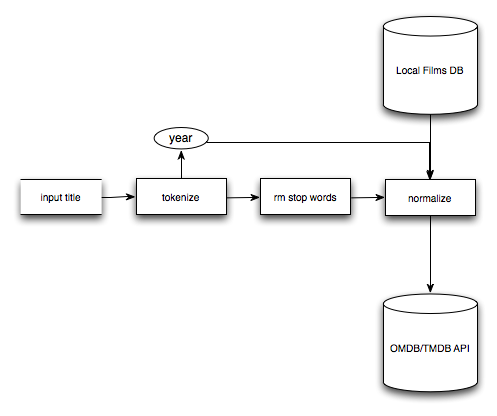
\includegraphics[scale=0.90]{title-identifier.png}
\caption{Movie Title Identification Algorithm. The title is tokenized, cleaned, and normalized before queried against external APIs.}
\label{fig:title-identifier}
\end{figure}


The title identification process was developed using the corpus of seed data. Using the filenames in the seed data, a set of stop words was compiled, eliminating many false positives. This method is computationally very inexpensive and has a high precision as \ref{sec:evaluation} shows. Extracting the year from the title string is also very effective in eliminating false positives due to film remakes. \\

Once the tokenized string is clean, an internal database of film names is used to find potential matches to query against online sources. The database is an in-memory SQLite database with on the order of 400,000 films. Putting this dataset in-memory allows an arbitrary amount of fuzzy matching (via the Python FuzzyWuzzy library), avoiding rate limiting issues when making requests to online sources and saves the network round-trip time. This also allows us to establish an element of ground truth locally before querying the online source. \\

\subsubsection{Credit Identifiers}
\label{sec:credit-identifier}

For many files in the initial corpus, titles were parsed successfully at a high rate since the data was relatively clean, however, the method is very brittle and can easily deliver false positives if a file is slightly misnamed or comes from a dirty source. To match entities more effectively, the credit identification method was implemented. This method performs optical character recognition (OCR) on the credits of a film and tries to extract actor names from the text. These names can then be queried against an online source and the intersection of the films in which the actors appear can be used to establish identity. \\

Figure \ref{fig:credit-identifier} outlines the credit identification algorithm. The film is cut to contain only the last five minutes of video and then a frame is generated every three seconds. Using the Tesseract library to perform OCR, raw text from each frame is extracted and then heuristically cleaned, reducing potential search tokens. Normalized text is generated by querying a local actors database to match a token to an actor and then a set of the actor's films are found from external APIs. The identifier returns a set of the intersection of films from the actors found. \\


\begin{figure}[H]
\center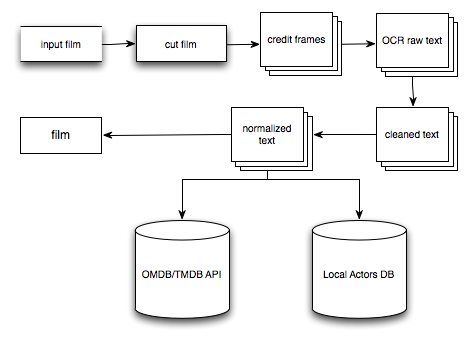
\includegraphics[scale=0.80]{credit-identifier.png}
\caption{Movie Credit Identification Algorithm. Outlines the flow from an input file to a set of potential film titles.}
\label{fig:credit-identifier}
\end{figure}


This method proved to be the most computationally expensive and required extensive optimizations to get an operational prototype implementation. The raw text from the OCR can produce many false results which cause the runtime of the fuzzy searching to reach the order of tens of minutes. To reduce this runtime, tokens are eliminated by several heuristics such as length and removing excluded characters. The fuzzy searching queries an in-memory SQLite database of known actor names and uses the Python FuzzyWuzzy library to score matches. \\

Some optimizations for this fuzzy matching process were first trying an exact match and then restricting the number of choices by finding the intersection of matches between first and last name instead of searching for a first name last name string together. The tokens extracted from the credit frames are queried against a local datastore of actor names for the same performance reasons as the title identifier. This ground truth data was scraped from the TMDB and OMDB APIs and contains approximately 450,000 actor names. \\

Since the credit frames are ordered with the leading actors first, another optimization was to perform the OCR in a streaming fashion since an intersection of a single film can likely be found within the first several frames which contain the leading actors. This also greatly reduces the amount of OCR and string processing that has to be performed. The largest remaining bottleneck was in the fuzzy matching, moving this implementation to a compiled language may show better results since the performance costs will be much lower. \\

\section{Evaluation}
\label{sec:evaluation}

The system was tested by ingesting two different sets of seed data totaling approximately 2 TB consisting entirely of movie entity files. We begin by discussing the overall performance of the system on the seed data and then analyzing the performance and accuracy of the title and credit identifiers. Due to the extended running time across the entire dataset, the system was only able to be tested fully once. There is high potential in future work for improving the performance with minor modifications to address the issues that we discovered. \\

This data set consisted of approximately 1000 entities, of which 702 of the jobs completed. In this first iteration of the system a single entity was expected for each queued job, so many of the failed jobs were due to multiple files being queued for a single job. The seed data contained many series or trilogies of films which were grouped together causing multiple files to be contained in what was believed to be one entity. In addition, some of the jobs failed since the film was split into two files. Future iterations of the handler would be more robust to determine if multiple entities were present (such as a series) or if the two files should be joined into one. \\

The runtime of the entire corpus took approximately 20 hours. This runtime encompasses the entire process of queuing jobs, computing the md5 hash, audio fingerprint, title identification, and credit identification. The system was run on an AMD A6-6400K 1.8GHz APU with Radeon(tm) HD Graphics and 4GB of RAM and 4 worker processes to consume jobs. On average, the deduplication process took 55.21 seconds to run, with the audio fingerprint computation taking almost the entire computation time. \\

%------------------------------------------------
\subsection{Identifiers}
\label{sec:identifiers-performance}
Using the output logs of The Librarian and the data from the metadata store, we found that the title identifier ran on average in 15.29 seconds. This time includes the entire process of fuzzy matching and network requests to outside sources. The credit identifier took 231.53 seconds on average from start to finish. Out of the 702 entities successfully processed, only 232 were identified. \\

184 of these entities were identified by the title identifier, and 67 were found by the credit identifier. 19 entities were successfully matched using both identification methods. The 35\% success rate is significantly lower than expected, however, with minor modifications to the system, we believe this rate can be greatly increased. \\

A possible reason for the low identification rate is that some of the heuristics are too stringent. For both credit and title matching, making less stringent heuristics will likely yield a higher identification rate. This would entail a larger search of possible tokens or lowering the threshold score of a fuzzy match. The scope of the project did not allow for fine tuning of the identification algorithms -- many of the design choices were made with limited training data examples. For credit identification, it is also possible that some credit sequences are longer than 5 minutes, in which case it is unlikely that a match would be found with the less well known actors. \\

Perhaps the main reason for the small number of successful identifications is the use of local ground truth data. Both the title and credit identifiers use local databases to normalize their queries before contacting an external API. Due to the number of queries on average (up to several thousand for fuzzy credit matching), this was a necessary optimization for this implementation. The problem with this is the local store is now a bottleneck for the search, since a valid string may be invalidated if the local store is missing an entry. \\

%------------------------------------------------

\section{Future Work}
\label{sec:future-work}

\subsection{Open Sourcing}
\label{sec:open-sourcing}
The Librarian was designed to be easily extended to additional entity types. Using the existing data pipeline, The Librarian handler classes can be added to identify text or audio files, and TV shows. Open sourcing the project is the main goal for future work. Once open sourced, developers can implement additional handlers for arbitrary entity types. The data pipeline provides the framework to process jobs in parallel and aggregate results in a datastore. A distributed version of this system is also an option to further parallelize the data processing. Because of the queue styled design, worker nodes can report to a single master to receive a job and perform the identification on the entity at a remote worker node after retrieving it from the source. \\

\subsection{Clients}
\label{sec:clients}
Another design feature of The Librarian was to allow clients to be built upon it. Some possible clients would allow entity gathering, a crowd sourcing resolution layer, or a media display server. \\

An entity gathering client would support receiving a link to a file, for example from Dropbox or a torrent file and then presenting this file to The Librarian for identification. Such a client fits the initial motivation for building The Librarian since the client would allow many users to add to a media store with large updates or incremental additions to a data set. \\

Another important client would be a crowd sourcing interface. This client also fits the model of many users accessing and adding to a media corpus. Identifiers can return multiple results for a single entity since matching is not guaranteed to be unique. For example, with title identification, if no year is specified, all remakes of the movies are potential matches. For credit identification the intersection of the actors is not guaranteed to be one. \\

Once The Librarian ingests a dataset, building a media server on top of it would be simple. A client can query the metadata store for any type of metadata that is held. One can imagine a Netflix style interface where, once the data is identified, users can query on any parameters such as title, actor, genre, etc. \\

\subsection{Optimizations}
\label{sec:optimizations}
Many optimization are also necessary before open sourcing could be completed. The current implementation is in Python, which is not well suited for computationally expensive data processing. Moving heavy parts of the identification process, such as fuzzy matching, to a compiled language would result in a large performance increase. Within the identifiers there is also room for optimization by tightening some of the arbitrary parameters we have designated. For example, during credit identification if OCR is only performed on frames with a threshold percentage of black pixels, frames without credit text will not be unnecessarily processed. \\


%------------------------------------------------
\section{Conclusion}
\label{sec:conclusion}

The Librarian provides a framework for parallelized entity identification across media entities. The data pipeline allows handlers to be added to identify media entities by providing a series of identification methods which are able to establish ground truth. The system uses deduplication to find matches to an entity internally and identification methods to use external data to establish ground truth. \\

This implementation showed a proof of concept for the system by implementing a movie identification handler. The handler used hashing and audio fingerprinting to deduplicate entities and with title and credit identification methods to establish initial ground truth. On the initial seed data of 2 TB of movie files, the movie handler proved to be more successful than credit identification. \\

The future work will bring additional functionality to the system by providing more handlers and making the current methods more robust. Open sourcing the project is the final goal to allow others to build clients upon the system and provide an open way to automatically identify media entities. The code is publicly available at \url{https://github.com/joshblum/the-librarian} .\\

%------------------------------------------------


\end{document}